\documentclass[aps,prd,reprint,nofootinbib, superscriptaddress]{revtex4-1}
\usepackage{amsmath,amssymb, amsthm,amstext}
\usepackage{natbib}
\usepackage{graphicx}
\usepackage{color}
\usepackage{array, enumerate}
\usepackage{bm}
\usepackage{multirow}
\usepackage[breaklinks,colorlinks,citecolor=blue]{hyperref}


% Shorts
\def\nn{\nonumber}
\def\st{\sin\theta}
\def\ct{\cos\theta}
\def\sst{\sin^2\theta}
\def\cct{\cos^2\theta}
\def\Ap{A_\phi}
\def\Ar{A_{\phi,r}}
\def\Arr{A_{\phi,rr}}
\def\Am{A_{\phi,\mu}}
\def\Amm{A_{\phi,\mu\mu}}
\def\Ah{A_{\phi,\theta}}
\def\be{\begin{equation}}
\def\ee{\end{equation}}
\def\ben{\begin{eqnarray}}
\def\een{\end{eqnarray}}
\def\WH{\Omega_{\rm H}}
\def\e{{\bf e}}
\def\AHE{A_\phi^{\rm HE}}
\def\AEE{A_\phi^{\rm EE}}


\def\Alfven{Alfv\`en}


\begin{document}
\title{The force-free magnetosphere of a Kerr black hole: the role of boundary conditions}
\author{Zhen Pan}
\email{zhpan@ucdavis.edu}
\affiliation{Perimeter Institute for Theoretical Physics, Waterloo, Ontario N2L 2Y5, Canada}

\date{\today}

\begin{abstract}
    xx
\end{abstract}


\maketitle

\section{Introduction}

\section{basic equations}
\label{sec:basic}
In this paper, we adopt the Kerr-Schild
coordinate with the line element
\[
\begin{aligned}
ds^2 =
&-\left( 1-\frac{2r}{\Sigma} \right)dt^2 + \left( \frac{4
r}{\Sigma} \right) dr dt + \left(1+\frac{2r}{\Sigma} \right) dr^2 \\
&+ \Sigma d\theta^2 - \frac{4 a r \sin^2\theta}{\Sigma} d\phi dt
- 2 a \left(1+\frac{2r}{\Sigma}\right) \sin^2\theta d\phi dr     \\
& + \frac{\beta}{\Sigma} \sst d\phi^2
\end{aligned}
\]
where $\Sigma = r^2 + a^2 \mu^2$, $\Delta = r^2 -2r + a^2$,
$\beta = \Delta\Sigma + 2r(r^2 + a^2)$, and $a$ is the dimensionless BH spin.
In the force-free approximation, electromagnetic energy greatly exceeds that of matter.
Consequently, the force-free magnetospheres is governed by energy
conservation equation of electromagnetic field, or
conventionally called as the GS equation.
In the Kerr spacetime,
the axisymmetric and steady GS equation can be written in a compact form \cite{Pan2017}
\ben
\label{eq:GSg}
&&\phantom{+}
 \left[\Arr + \frac{\sst}{\Delta}\Amm \right]  \mathcal K(r,\theta; \Omega )\nn \\
&&
+\left[\Ar \partial_r^\Omega  +  \frac{\sst}{\Delta}\Am \partial_\mu^\Omega\right] \mathcal K(r,\theta; \Omega ) \nn \\
&&
+ \frac{1}{2}\left[\Ar^2 + \frac{\sst}{\Delta}\Am^2\right]  \Omega' \partial_\Omega \mathcal K(r,\theta; \Omega )\nn \\
&&
- \frac{\Sigma}{\Delta}II' = 0 \ ,
\een
with $\mathcal K(r,\theta; \Omega )= \left[\frac{\beta}{\Sigma}\Omega^2 \sst
-\frac{4ra}{\Sigma}\Omega \sst
-\left(1-\frac{2r}{\Sigma}\right)\right]$ being the LS function,
$\mu\equiv\ct$,  and  the primes designate  derivatives with respect to $A_\phi$.
$\partial_i^\Omega (i=r, \mu)$  denotes the partial derivative
with respect to coordinate $i$ with $\Omega$ fixed, and $\partial_\Omega$ is the derivative with
respect to $\Omega$.

\section{Uniform field solution}

\subsection{Boundary conditions}

\begin{subequations}
\begin{align}
    A_\phi(\mu = 1) &= 0,  \label{eq:bc1}\\
    \Am(\mu = 0, r > 2) &= 0, \label{eq:bc2}\\
    B^2-E^2 (\mu = 0, r_+ \leq r \leq 2) &=0.\label{eq:bc3}
\end{align}
\end{subequations}

where
\be
\begin{aligned}
B^2-E^2 &= \frac{1}{\Sigma \sst} \left[ -\mathcal{K} \left(\Ar^2 +\frac{\sst}{\Delta}\Am^2 \right)+\frac{\Sigma}{\Delta}I^2\right]\\
B^2+E^2 &= \frac{1}{\Sigma \sst} \left[ \left(\mathcal{K}+\frac{\Delta\Sigma}{\beta} \right) \left(\Ar^2 +\frac{\sst}{\Delta}\Am^2 \right)+\frac{\Sigma}{\Delta}I^2\right]\\
\end{aligned}
\ee
\be
\label{eq:nbc}
\int_{A_\phi^{\rm HE}}^{A_\phi^{\rm EE}} \frac{B^2-E^2}{B^2+E^2} dA_\phi \Big/ \left(A_\phi^{\rm EE}- A_\phi^{\rm HE}\right)  < 10^{-3}.
\ee
where ``HE" and ``EE" are short for Horizon-Equator and Ergosphere-Equator, respectively.

\subsection{Numerical method}
We aim to find a pair of $\Omega(A_\phi)$ and $I(A_\phi)$ satisfying the radiation condition
\be I = 2\Omega A_\phi, \label{eq:rad}\ee
and suitable $\Am(\mu =0, r_+\leq r \leq 2)$
enabling the boundary condition (\ref{eq:bc3}).

1. We choose an initial guess for the field configuration, $\Omega(\Ap)$ and equator boundary condition as follows
\begin{subequations}
\begin{align}
    \Ap &= r^2 \sst,  \label{eq:gss1} \\
    \Omega & = 0.5\WH\left(1-\Ap/\AHE\right), \label{eq:gss2}\\
    \Am(\mu =0, r_+\leq r \leq 2) & = -1\times (r/r_+)^3. \label{eq:gss3}
\end{align}
\end{subequations}

2. We evolve the GS equation and find $II'$ enabling smooth field lines across the LS
\cite[see][for details]{Contopoulos2013, Nathanail2014, Pan2016a}.

3. Usually the current $I$ found in Step 2 neither satisfies the radiation condition (\ref{eq:rad})
nor enables the boundary condition (\ref{eq:bc3}). We find it is possible to adjust
$\Am(\mu = 0, r_+ \leq r\leq 2)$ as follows
\be
 A_{\phi,\mu\rm new}  = A_{\phi,\mu \rm old} + \zeta_1\times[2\Omega\Ap(2\Omega\Ap)' -II'],
\ee
enabling the radiation condition (\ref{eq:rad}) for
$A_\phi\in [A_\phi^{\rm HE}, A_\phi^{\rm EE}]$, where $\zeta_1$ is an
empirical step size.

4. The final step is to adjust  $\Omega(\Ap < \AHE)$ enabling  the radiation condition (\ref{eq:rad})
 for $A_\phi < A_\phi^{\rm HE}$ and  to adjust $\Omega(\AHE \leq \Ap \leq \AEE)$
 enabling the boundary condition (\ref{eq:bc3}) for $\Ap \in [\AHE, \AEE]$.
 The first part is straightforward, i.e.,
 \be
\Omega_{\rm new}(\Ap < \AHE) = \frac{I}{2\Ap},
 \ee
 and the second part can be realized by
 \be
\Omega_{\rm new}  = \Omega_{\rm old} - \zeta_2\times\frac{\Delta (B^2-E^2)}{2\Ap}\Big|_{\mu=0, r_+\leq r \leq 2}
 \ee
 where $\zeta_2$ is again an empirical step size, and we have multiplied factor $\Delta$
 to avoid numerical difficulty in the vicinity of the event horizon. To avoid unphysical discontinuity in the angular
 velocity at $\AHE$, we fit $\Omega_{\rm new}(\Ap)$ via a fifth-order polynomial.

 5. For the new angular velocity $\Omega_{\rm new}(\Ap)$ obtained in Step 4, we repeat step 2 to step 4,
 until the numerical prescription (\ref{eq:nbc}) is satisfied.

\begin{figure}
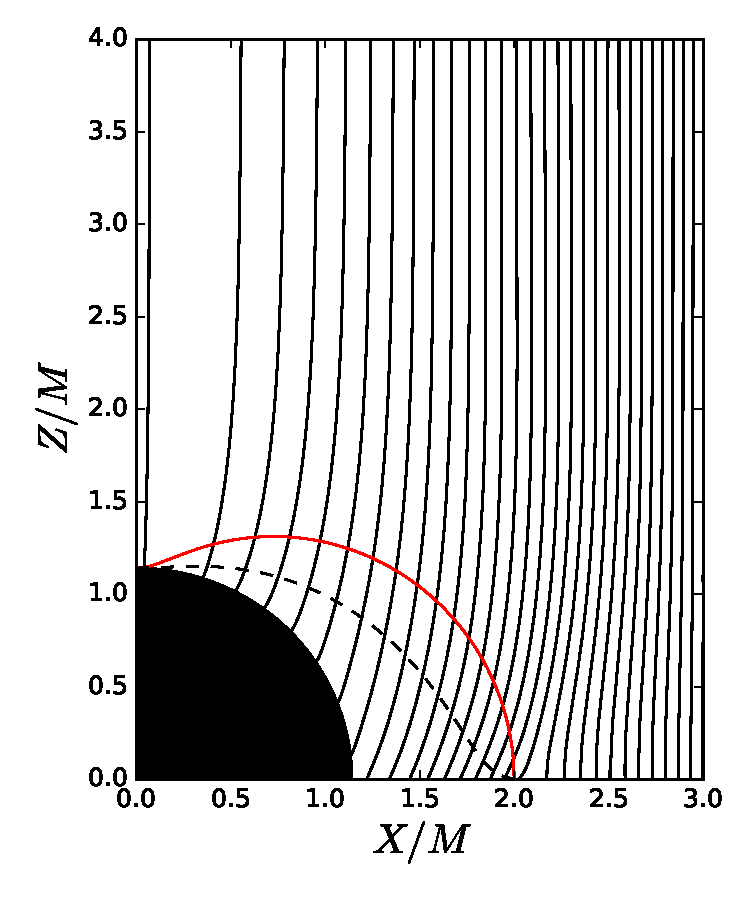
\includegraphics[scale=0.55]{f1}
\caption{\label{fig:field_lines} The configuration of field lines for the magnetosphere of a Kerr BH with spin $a=0.99$,
where the solid/red line is the ergosphere and the dashed/black line is the LS, both of which intersect with
the equator at $r=2 M$. }
\end{figure}

\begin{figure}
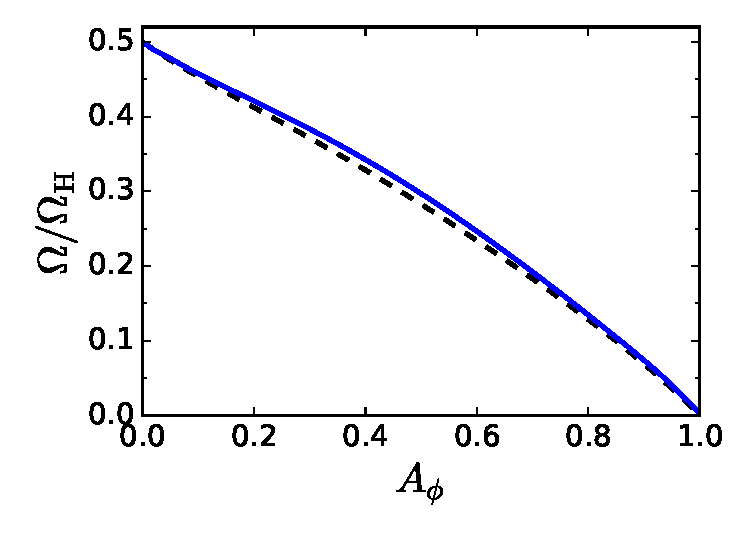
\includegraphics[scale=0.6]{f2}
\caption{\label{fig:omega} $a=0.99$}
\end{figure}


\bibliography{ms}


\end{document}
